\documentclass[conference,10pt]{IEEEtran}
\IEEEoverridecommandlockouts

\usepackage{amsmath}
\usepackage{graphicx}
\usepackage{booktabs}
\usepackage{multirow}
\usepackage{array}
\usepackage{xcolor}
\usepackage{url}
\usepackage{placeins}
\usepackage[hidelinks]{hyperref}

% let floats sit close to their text
\renewcommand{\topfraction}{0.95}
\renewcommand{\bottomfraction}{0.9}
\renewcommand{\textfraction}{0.05}
\renewcommand{\floatpagefraction}{0.85}
\renewcommand{\dbltopfraction}{0.95}
\renewcommand{\dblfloatpagefraction}{0.85}
\setcounter{topnumber}{3}
\setcounter{bottomnumber}{2}
\setcounter{totalnumber}{6}
\setcounter{dbltopnumber}{2}

\graphicspath{{../figures/}{../old/figures/final/}}
\newcommand{\cc}[1]{\texttt{#1}}
\newcommand{\pct}{\,\%}
\setlength{\tabcolsep}{4pt}

\begin{document}

\title{ML-Driven PVT-Variation-Aware Leakage Estimation\\for a 16\,nm HP 8-bit Parity Checker}

\author{\IEEEauthorblockN{Bhargav (2023112014),
Nitin (2023112026),
Karthik (2023102009),
Roshan Lal (2023102010)}
\IEEEauthorblockA{Digital VLSI Design --- Course Project\\
Model file: 16nm\_HP $\cdot$ $V_{DD}=0.9$\,V $\cdot$ Test circuit: 8-bit parity checker}}

\maketitle

\begin{abstract}
We estimate the leakage of CMOS gates and of an 8-bit parity checker under process, voltage and
temperature (PVT) variation with machine-learning (ML) models of single transistors instead of
circuit-level SPICE. Four models (NMOS/PMOS, ON/OFF) predict the four terminal currents from
360,000 single-transistor ngspice simulations of the PTM 16\,nm high-performance card. An averaged
Gaussian process on physics-based features reaches a median error of 0.14--0.28\pct{} on the test
set for every current above $10^{-11}$\,A. From these models alone, the leakage of INV, NAND2, NOR2,
AND2 and OR2 (18 input cases $\times$ 200 PVT corners with random NMOS/PMOS widths) is predicted
with 98.69\pct{} mean accuracy using SPICE node voltages and 98.15\pct{} with node voltages also
predicted by the models. The parity checker (256 vectors $\times$ 200 corners), composed from
NAND2 predictions, reaches 96.91\pct{} and 97.08\pct{}; we show that the remaining circuit error
is almost entirely the $-2.2$\pct{} bias of the prescribed gate-summation method itself.
\end{abstract}

% =====================================================================
\section{Setup}

Table~\ref{tab:setup} lists the assignment and tools. Accuracy is defined, as in the project
document, as $100\pct - \overline{|e|}$ with the relative error $e=(I_{ML}-I_{SPICE})/I_{SPICE}$;
we also report the median and 95th-percentile (p95) of $|e|$ and the \emph{bias}, the median of
the signed error.

\begin{table}[!htb]
\caption{Assignment and tools}
\label{tab:setup}
\centering
\begin{tabular}{@{}ll@{}}
\toprule
Model file & PTM~\cite{ptm} \cc{16nm\_HP.pm} (BSIM4~\cite{bsim4}, level 54)\\
Nominal $V_{DD}$ & 0.9\,V (sampled 0.81--0.99\,V)\\
Channel length & $L=16$\,nm; widths 16--128\,nm ($1$--$8\,L_{min}$)\\
Test circuit & 8-bit parity checker (28 NAND2, 112 FETs)\\
Simulator & ngspice-36~\cite{ngspice}, Ubuntu 22.04\\
Software & Python 3.10, scikit-learn 1.7~\cite{sklearn}, numpy 2.2,\\
 & pandas 2.3, scipy 1.15, LightGBM~\cite{lgbm}\\
\bottomrule
\end{tabular}
\end{table}

\textbf{Leakage definition.} The leakage of a gate or circuit is the total current drawn from
everything held at logic~1: the $V_{DD}$ supply current plus the current into every input held at
$V_{DD}$, i.e.\ $I_{leak}=-\big(I(V_{DD})+\sum_{\text{inputs}=1} I(V_{in})\big)$. It equals the static
power divided by $V_{DD}$, and with it the leakage of a circuit is the sum of the leakages of its
gates. The same definition is used in SPICE and ML.

\textbf{Width setup.} The project fixes the transistor widths of the datasets
($1$--$8\,L_{min}$) but not of the gates. Following the TAs' advice to vary the widths, each of the
200 corners draws one NMOS width $W_n$ and one PMOS width $W_p$, uniform in 16--128\,nm, shared by
all NMOS and all PMOS of the gates and of the circuit at that corner. The gates and the circuit are
thus tested over the whole trained width range, including unbalanced pull-up/pull-down strengths.

% =====================================================================
\section{Data Generation}

\subsection{Sampling and netlists}
For each case (NMOS ON, NMOS OFF, PMOS ON, PMOS OFF) we drew 10,000 samples, every parameter
uniform and independent: $V_{DD}$ first (0.81--0.99\,V), then $V_d, V_s\in[0,V_{DD}]$,
$W\in[16,128]$\,nm, $T\in[-40,125]^\circ$C, and \cc{vth0}, \cc{toxe}, \cc{ndep}, \cc{u0}, \cc{xj}
each within $\pm10\pct$ of the card's nominal value (separate values for NMOS and PMOS). The gate
and body voltages follow the case: $V_g=V_{DD}$ (NMOS ON, PMOS OFF) or 0, $V_b=0$ (NMOS) or
$V_{DD}$ (PMOS).

Each sample is one netlist: a copy of the model card with the sample's five process parameters,
one DC voltage source per terminal, \cc{.options gmin=1e-18 abstol=1e-18 reltol=1e-6 vntol=1e-9},
and an \cc{.op} analysis. One ngspice process runs hundreds of netlists back to back, four
processes in parallel (10,000 runs in $\approx$30\,s); no run failed. The currents are the raw
ngspice source currents (positive = out of the device).

Each case is stored as one CSV with the document's columns \cc{vdd, temp, w, vd, vs, vg, vb,
vth0, toxe, ndep, u0, xj, id, ig, is, ib} (SI units).

The document allows more samples. We added 80,000 training rows per case from the same generator
with new, disjoint seeds, so the final models train on 87,000 rows per case.

\subsection{Split}
Each 10,000-row dataset is split 70/15/15 (7,000 / 1,500 / 1,500) with seed 42. Validation and
test are always these original rows; the extra rows are used for training only.

\subsection{Data check}
\textbf{Kirchhoff check.} Table~\ref{tab:kcl} gives $|I_d+I_g+I_s+I_b|$ for each case. All
residuals are at ngspice's numerical resolution and below 0.08\pct{} of any current above
10\,pA. Every parameter is inside its range, there are no duplicates, and the extra rows follow
the same distribution (KS test, all $p>0.05$).

\begin{table}[!htb]
\caption{Kirchhoff check per case: $|I_d+I_g+I_s+I_b|$ in A}
\label{tab:kcl}
\centering
\footnotesize
\begin{tabular}{@{}lccc@{}}
\toprule
 & \multicolumn{2}{c}{Dataset (10,000 rows)} & Extra rows (80,000)\\
\cmidrule(lr){2-3}\cmidrule(lr){4-4}
Case & Median & Max & Max\\
\midrule
NMOS ON & $2.1\times10^{-16}$ & $1.0\times10^{-14}$ & $1.0\times10^{-14}$\\
NMOS OFF & $4.9\times10^{-22}$ & $8.2\times10^{-18}$ & $4.7\times10^{-17}$\\
PMOS ON & $7.7\times10^{-17}$ & $9.9\times10^{-15}$ & $1.0\times10^{-14}$\\
PMOS OFF & $8.2\times10^{-17}$ & $1.3\times10^{-15}$ & $1.4\times10^{-15}$\\
\bottomrule
\end{tabular}
\end{table}

\textbf{Trend plots} (Fig.~\ref{fig:trends}) agree with device physics: the OFF current rises
$\approx$6$\times$ (NMOS) and 3$\times$ (PMOS) from $-40$ to $125^\circ$C, falls exponentially with
$|$\cc{vth0}$|$ ($\approx$10$\times$ per 0.1\,V), and the gate current falls exponentially with
\cc{toxe}. The left panels show the random data, the right panels a clean SPICE sweep at nominal
values.

\begin{figure}[!htbp]
\centering
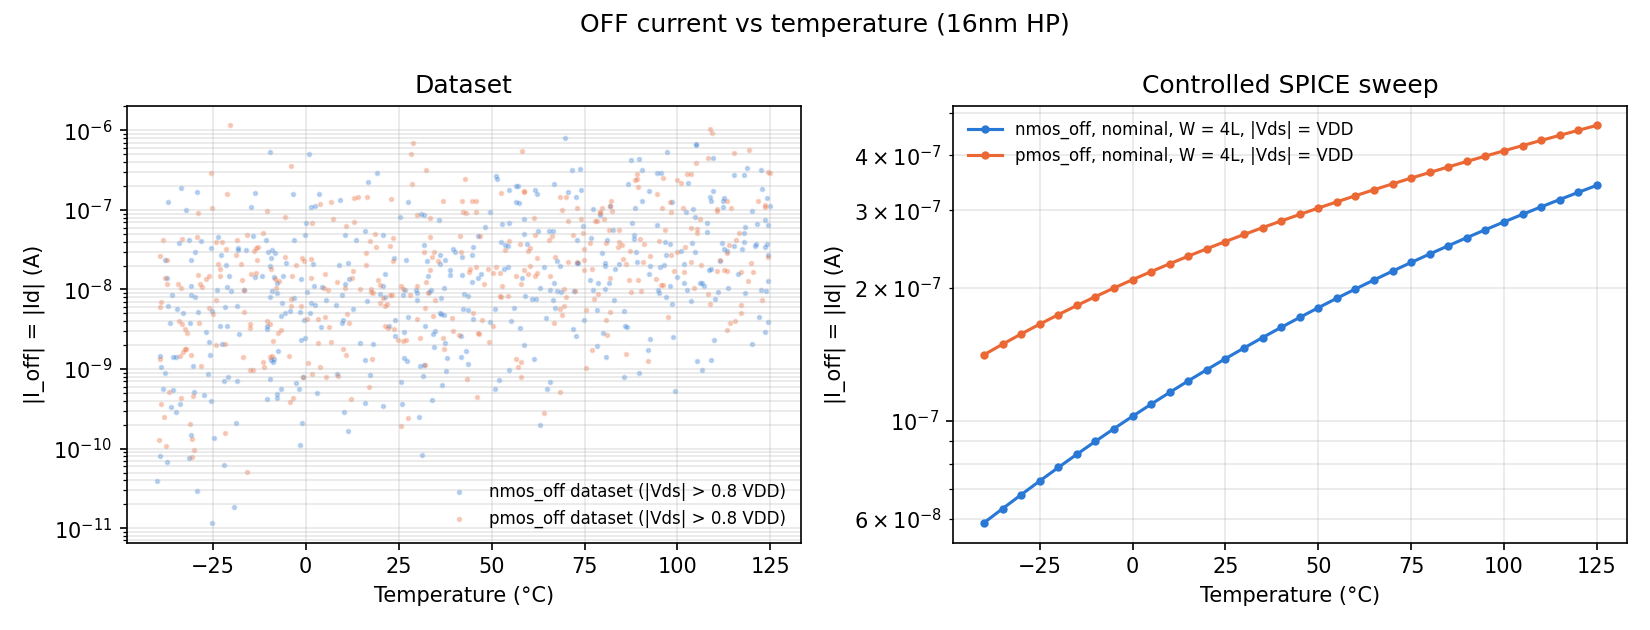
\includegraphics[width=\columnwidth]{trend_ioff_vs_temp.png}\\[1pt]
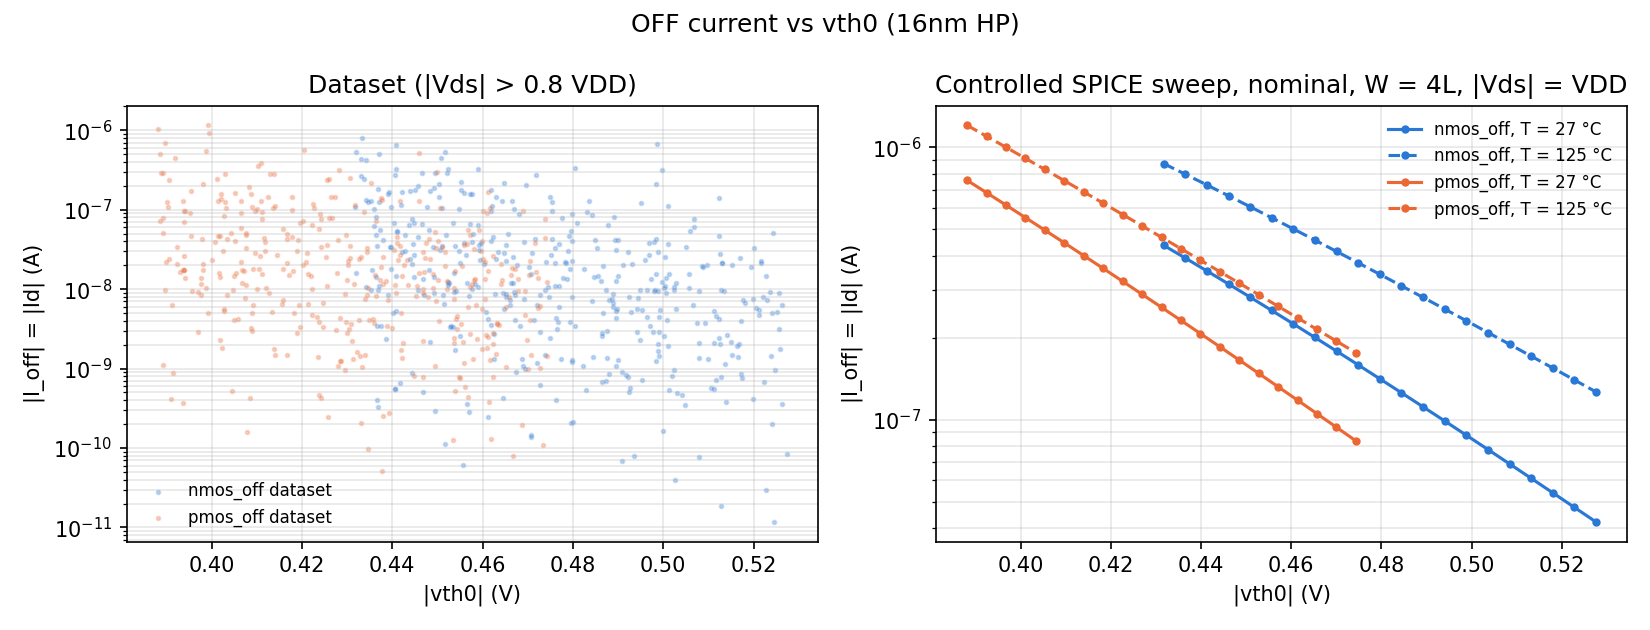
\includegraphics[width=\columnwidth]{trend_ioff_vs_vth0.png}\\[1pt]
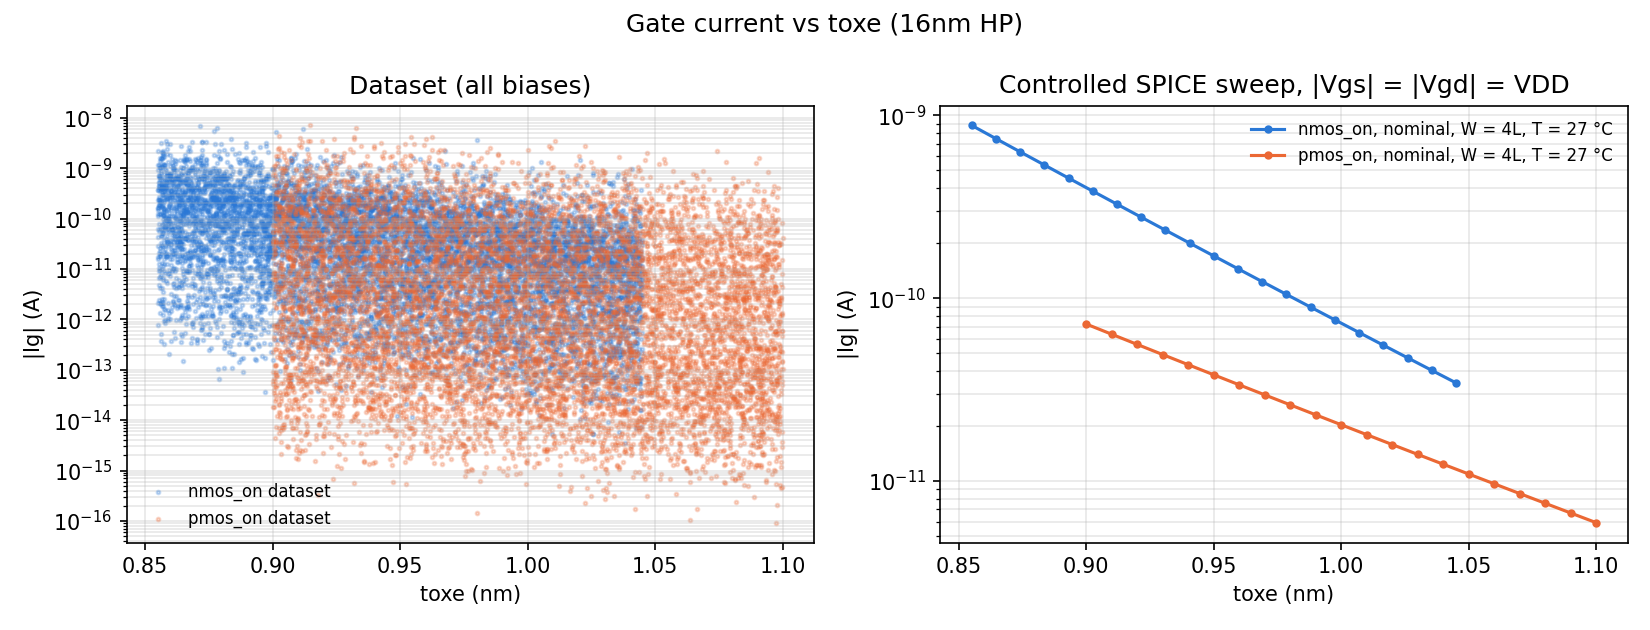
\includegraphics[width=\columnwidth]{trend_ig_vs_toxe.png}
\caption{Data check, top to bottom: OFF current vs temperature, OFF current vs \cc{vth0}, gate current vs \cc{toxe}. Left panels: random dataset; right panels: SPICE sweep at nominal values.}
\label{fig:trends}
\end{figure}

% =====================================================================
\section{Transistor Models}

\subsection{Preprocessing}
Leakage currents span 13 decades and some currents change sign, so all models share the
following preprocessing:
\begin{enumerate}
\item \emph{Symmetric frame}: the higher of $V_d,V_s$ is called ``hi'' and the lower ``lo''; the
channel current then always flows the same way.
\item \emph{Log target}: each model predicts $\ln(|I|/W)$; an error of 0.01 is $\approx$1\pct{} at
any current level.
\item \emph{KCL}: the one current that can change sign is computed as minus the sum of the other
three, so every prediction satisfies KCL exactly.
\item \emph{Physics features}: the variables of the BSIM sub-threshold expression
$I\propto[1-e^{-V_{DS}/V_t}]\,e^{(V_{GS}-V_{th})/nV_t}$: $V_{gs}/V_t$, $V_{gd}/V_t$,
$V_{ds}/V_t$, $|\cc{vth0}|/V_t$, $1/V_t$, $\ln(1-e^{-V_{ds}/V_t})$ (clamped at
$V_{ds}=2$\,mV), $\ln W$ and the five process parameters, standardised. The ON models also get the
plain $V_{gs},V_{gd},V_{ds}$, because gate tunnelling depends on the oxide voltage, not on $kT/q$.
\end{enumerate}

\subsection{Model types}
We compared four types on the 7,000-row training split:
\begin{itemize}
\item \emph{Polynomial ridge}: degree-3 polynomial, $\alpha=10^{-4}$.
\item \emph{LightGBM}: 5,000 trees, learning rate 0.02, 15 leaves.
\item \emph{MLP}: 3 hidden layers $\times$ 64 tanh units, Adam, early stopping.
\item \emph{Gaussian process (GP)}~\cite{gp}: linear mean plus an ARD RBF kernel whose hyperparameters are
fitted on 2,000 points, then an exact GP on all training points.
\end{itemize}

\begin{table*}[!t]
\caption{Model comparison on the validation set (7,000 training rows): $R^2$ of $\log_{10}|I|$, median and p95 relative error (\%) per current}
\label{tab:modelcmp}
\centering
\footnotesize
\begin{tabular}{@{}ll ccc ccc ccc ccc c@{}}
\toprule
 & & \multicolumn{3}{c}{$I_d$} & \multicolumn{3}{c}{$I_g$} & \multicolumn{3}{c}{$I_s$} & \multicolumn{3}{c}{$I_b$} & Mean of\\
\cmidrule(lr){3-5}\cmidrule(lr){6-8}\cmidrule(lr){9-11}\cmidrule(lr){12-14}
Case & Model & $R^2$ & med & p95 & $R^2$ & med & p95 & $R^2$ & med & p95 & $R^2$ & med & p95 & medians\\
\midrule
NMOS ON & Poly ridge & 0.9971 & 12.3 & 38.4 & 0.9950 & 6.98 & 28.4 & 0.9970 & 12.3 & 38.7 & 0.9944 & 13.1 & 43.8 & 11.2\\
 & LightGBM & 0.9987 & 3.65 & 28.3 & 0.9982 & 5.76 & 20.3 & 0.9985 & 3.65 & 27.5 & 0.9973 & 8.64 & 29.3 & 5.42\\
 & MLP & 0.9992 & 2.76 & 15.5 & 0.9990 & 3.58 & 13.9 & 0.9989 & 2.90 & 15.5 & 0.9996 & 3.15 & 11.0 & 3.10\\
 & \textbf{GP} & 0.9995 & \textbf{0.52} & \textbf{4.16} & 0.9996 & \textbf{0.37} & \textbf{5.89} & 0.9991 & \textbf{0.50} & \textbf{4.03} & 1.0000 & \textbf{0.49} & \textbf{2.98} & \textbf{0.47}\\
\midrule
NMOS OFF & Poly ridge & 0.9000 & 28.6 & 322 & 0.9996 & 1.13 & 4.96 & 0.9104 & 26.4 & 326 & 0.9412 & 21.1 & 49.1 & 19.3\\
 & LightGBM & 0.9760 & 9.04 & 69.2 & 0.9986 & 3.34 & 11.9 & 0.9789 & 9.01 & 65.1 & 0.9842 & 1.12 & 21.5 & 5.63\\
 & MLP & 0.9944 & 3.53 & 24.5 & 0.9992 & 1.63 & 9.19 & 0.9953 & 3.46 & 24.3 & 0.9835 & 1.69 & 24.5 & 2.58\\
 & \textbf{GP} & 0.9969 & \textbf{0.66} & \textbf{10.5} & 0.9990 & \textbf{0.002} & \textbf{0.02} & 0.9959 & \textbf{0.62} & \textbf{8.88} & 0.9798 & \textbf{0.18} & \textbf{21.4} & \textbf{0.37}\\
\midrule
PMOS ON & Poly ridge & 0.9968 & 10.6 & 32.7 & 0.9946 & 10.7 & 44.4 & 0.9967 & 10.6 & 32.6 & 0.9936 & 13.6 & 50.6 & 11.4\\
 & LightGBM & 0.9978 & 3.35 & 26.9 & 0.9964 & 10.3 & 40.6 & 0.9977 & 3.41 & 27.1 & 0.9976 & 9.12 & 31.4 & 6.54\\
 & MLP & 0.9983 & 5.53 & 13.5 & 0.9976 & 2.78 & 14.3 & 0.9983 & 5.51 & 13.9 & 0.9996 & 3.24 & 13.6 & 4.27\\
 & \textbf{GP} & 0.9982 & \textbf{0.54} & \textbf{3.27} & 1.0000 & \textbf{0.10} & \textbf{1.01} & 0.9981 & \textbf{0.52} & \textbf{3.19} & 1.0000 & \textbf{0.42} & \textbf{2.54} & \textbf{0.40}\\
\midrule
PMOS OFF & Poly ridge & 0.9679 & 14.4 & 331 & $-$0.076 & 51.9 & 1216 & 0.9501 & 16.2 & 1257 & 0.9593 & 20.1 & 51.3 & 25.6\\
 & LightGBM & 0.9714 & 19.1 & 280 & $-$0.077 & 35.0 & 1268 & 0.9514 & 19.5 & 1187 & 0.9886 & 1.42 & 21.1 & 18.8\\
 & MLP & 0.9736 & 16.2 & 282 & $-$0.077 & 20.2 & 1283 & 0.9549 & 17.4 & 1240 & 0.9850 & 5.22 & 30.5 & 14.8\\
 & \textbf{GP} & 0.9608 & \textbf{9.62} & 370 & 0.138 & \textbf{2.57} & \textbf{72.5} & 0.9552 & \textbf{9.72} & 1137 & 0.9876 & \textbf{0.50} & \textbf{20.1} & \textbf{5.60}\\
\bottomrule
\end{tabular}
\end{table*}

\subsection{Comparison and choice}
Table~\ref{tab:modelcmp} is the comparison on the validation set. The GP has the lowest median
error for every current of every case, 2--10$\times$ below the next best, because SPICE currents
are smooth, noise-free functions of the inputs, which a GP with a per-input length scale
interpolates almost exactly. The PMOS OFF $I_g$ and the large p95 values of the OFF cases come from
currents near $10^{-14}$\,A: about two thirds of the PMOS OFF values sit at the junction/noise
floor, where ngspice resolves currents only in steps of $\approx2\times10^{-16}$\,A, so the $R^2$
of $\log|I|$ is low for every model type. These currents are over 1,000$\times$ below any gate
leakage.

\textbf{Final models.} The chosen model type is the GP, improved in three ways, each chosen on the
transistor validation split only:
\begin{enumerate}
\item \emph{All 87,000 rows} through an \emph{averaged GP}: the kernel is fitted once per current
on 2,000 points, then one exact GP is trained on each of 9 disjoint slices of $\le$9,700 rows, and
the predictions are averaged (an exact GP on 87,000 rows would need $\approx$60\,GB).
\item \emph{Two experts} for the OFF cases, split where the channel stops dominating
(30\pct{} of $V_{DD}$ for PMOS, 12.5\pct{} for NMOS); currents below $3\times10^{-15}$\,A are not
used for training.
\item The plain-voltage features for the ON cases (above).
\end{enumerate}
A stronger MLP ensemble on all 87,000 rows (3 seeds of per-current 3$\times$128 networks) gave
0.38--6.4\pct{} mean validation median against 0.26--3.9\pct{} for the GP in every case, and was
not used.

\begin{table}[!htbp]
\caption{Validation error of the final model type vs training rows per case (mean of the four per-current medians, \%)}
\label{tab:size}
\centering
\footnotesize
\begin{tabular}{@{}lcccc@{}}
\toprule
Rows & NMOS ON & NMOS OFF & PMOS ON & PMOS OFF\\
\midrule
2,000 & 0.67 & 0.76 & 0.52 & 6.94\\
4,000 & 0.51 & 0.49 & 0.38 & 6.81\\
7,000 & 0.41 & 0.36 & 0.33 & 5.68\\
27,000 & 0.32 & 0.27 & 0.28 & 5.12\\
47,000 & 0.30 & 0.29 & 0.27 & 3.97\\
\textbf{87,000} & \textbf{0.31} & \textbf{0.26} & \textbf{0.27} & \textbf{3.94}\\
\bottomrule
\end{tabular}
\end{table}

\begin{figure}[!htbp]
\centering
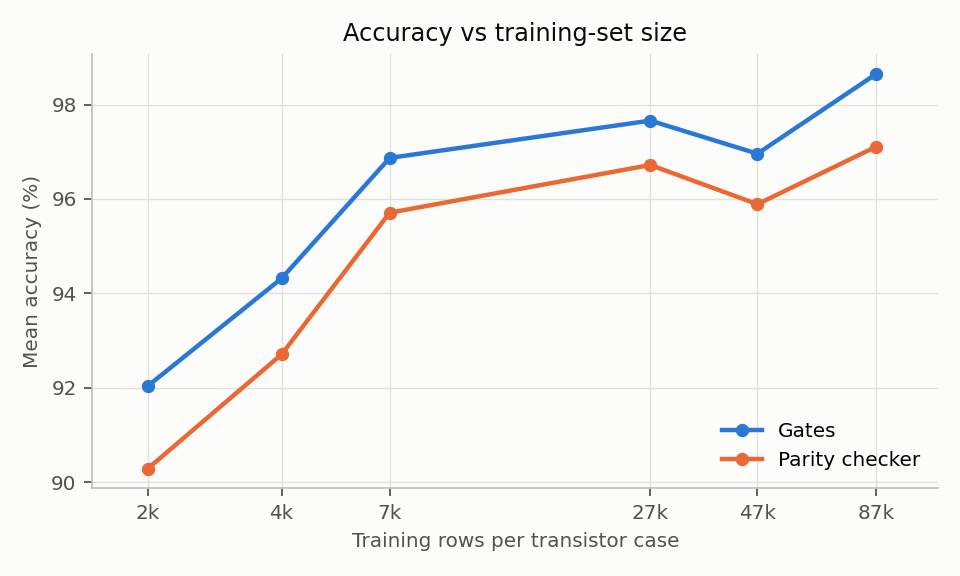
\includegraphics[width=\columnwidth]{size_study.png}
\caption{Gate and parity-checker accuracy vs training rows per case for the final model type (development study).}
\label{fig:size}
\end{figure}

\textbf{Dataset size.} Table~\ref{tab:size} shows the validation error for 2,000 to 87,000
training rows. It falls steadily up to $\approx$27,000 rows; beyond that mainly PMOS OFF keeps
improving (5.1\pct{} to 3.9\pct). In our gate-level development study (Fig.~\ref{fig:size}), gate
accuracy kept rising up to 87,000 rows: gates depend on a few sparsely sampled operating points
(e.g.\ an OFF PMOS holding the full supply), which need many random samples. We therefore use all
87,000 rows.

\begin{table}[!t]
\caption{Final models on the test set (1,501 rows per case): median / p95 relative error (\%) and $R^2$ of $\log_{10}|I|$}
\label{tab:test}
\centering
\footnotesize
\setlength{\tabcolsep}{3pt}
\begin{tabular}{@{}lcccc c@{}}
\toprule
Case & $I_d$ & $I_g$ & $I_s$ & $I_b$ & $|I|\ge10^{-11}$\,A\\
\midrule
NMOS ON & 0.36 / 2.4 & 0.16 / 2.4 & 0.36 / 2.5 & 0.38 / 2.0 & 0.26 / 1.8\\
NMOS OFF & 0.48 / 6.5 & 0.00 / 0.01 & 0.46 / 8.3 & 0.13 / 23 & 0.14 / 2.3\\
PMOS ON & 0.36 / 1.9 & 0.06 / 0.4 & 0.36 / 1.8 & 0.35 / 2.0 & 0.27 / 1.6\\
PMOS OFF & 7.0 / 307 & 3.1 / 70 & 7.3 / 1114 & 0.40 / 19 & 0.28 / 3.3\\
\midrule
\multicolumn{6}{@{}l}{$R^2$ (worst current): NMOS ON 0.9996, NMOS OFF 0.971,}\\
\multicolumn{6}{@{}l}{PMOS ON 0.9997, PMOS OFF 0.948}\\
\bottomrule
\end{tabular}
\end{table}

\textbf{Test results} (Table~\ref{tab:test}, Fig.~\ref{fig:pred}). On all currents of at least
$10^{-11}$\,A, the range that matters for gate leakage ($\ge3\times10^{-11}$\,A), the median error
is 0.14--0.28\pct{} for all four models. The large PMOS OFF numbers come entirely from the
$\sim10^{-14}$\,A noise floor: in Fig.~\ref{fig:pred} every PMOS OFF current above
$\sim10^{-12}$\,A lies on the diagonal. Validation and test stay at the prescribed 1,500 rows
so that every model and training size is scored on the same data; on 2,000 further fresh samples
per case (seeds 9000--9003) the median error for currents $\ge10^{-11}$\,A was 0.15--0.26\pct,
confirming the test-set figures.

\begin{figure*}[!t]
\centering
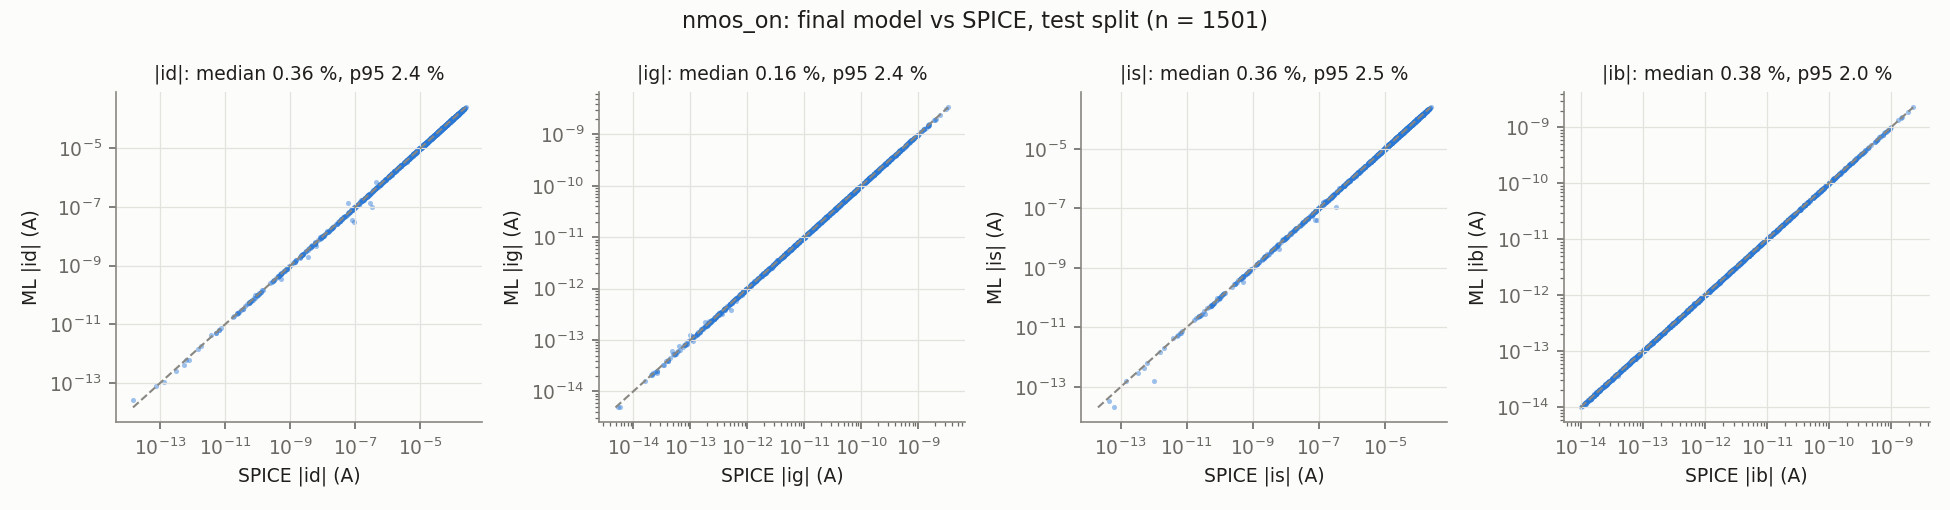
\includegraphics[width=0.86\textwidth]{pred_vs_spice_nmos_on.png}\\[2pt]
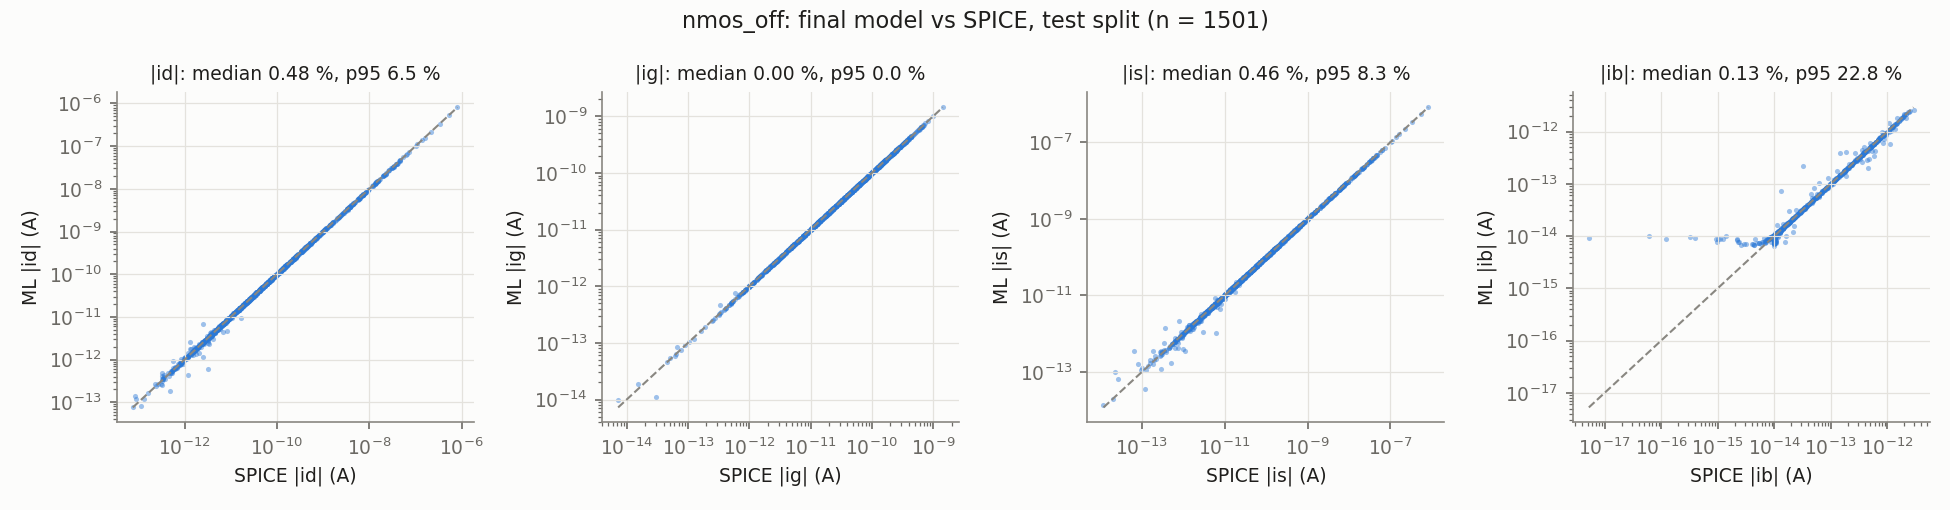
\includegraphics[width=0.86\textwidth]{pred_vs_spice_nmos_off.png}\\[2pt]
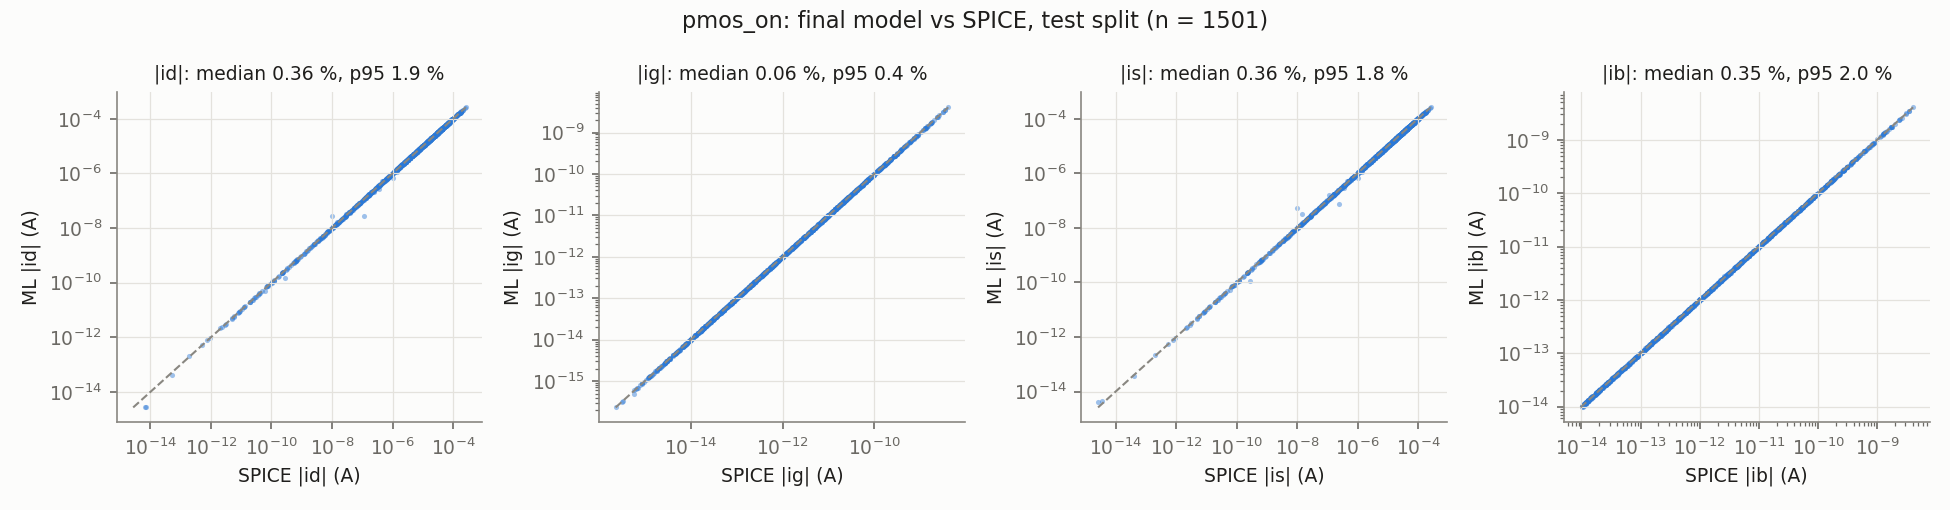
\includegraphics[width=0.86\textwidth]{pred_vs_spice_pmos_on.png}\\[2pt]
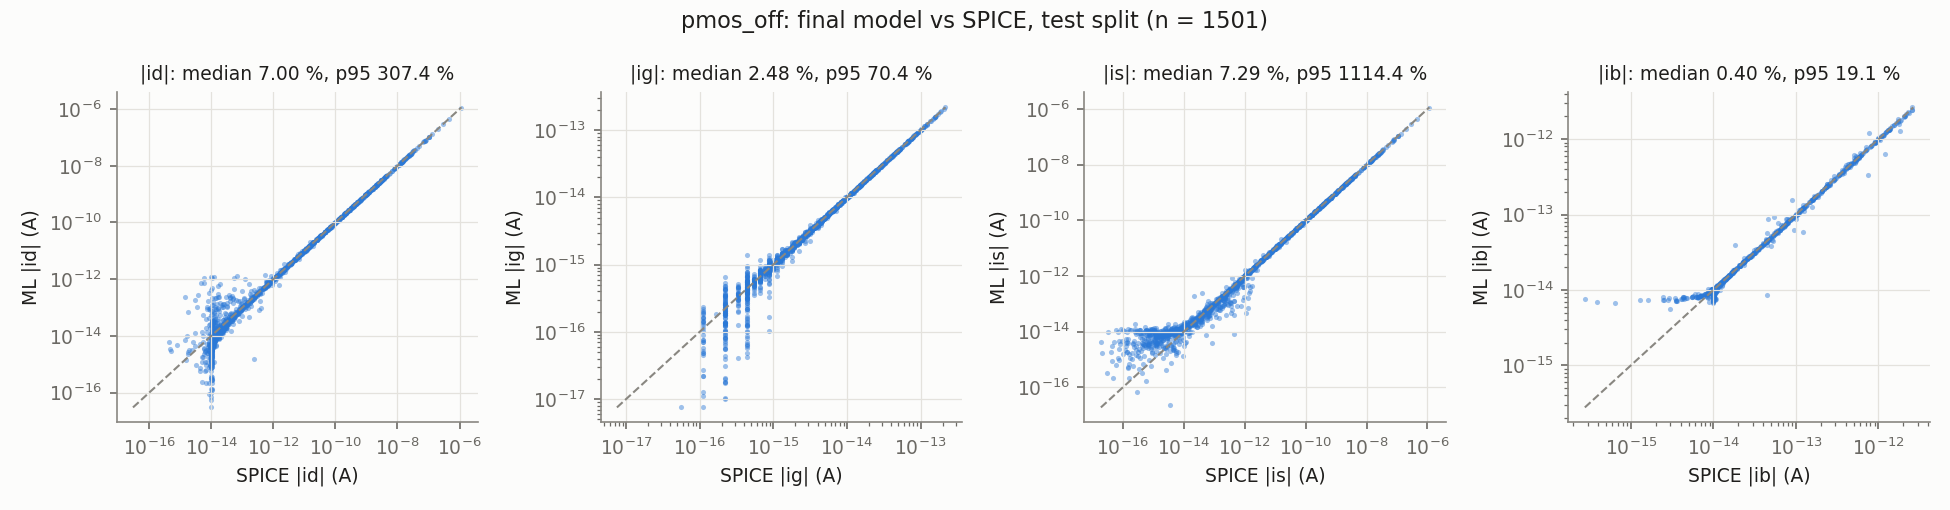
\includegraphics[width=0.86\textwidth]{pred_vs_spice_pmos_off.png}
\caption{Predicted vs SPICE terminal currents of the final models on the test set (rows: NMOS ON, NMOS OFF, PMOS ON, PMOS OFF). The scatter at the bottom of the OFF panels is the $\sim10^{-14}$\,A noise floor; the vertical stripes in PMOS OFF $I_g$ are ngspice's resolution steps.}
\label{fig:pred}
\end{figure*}

% =====================================================================
\section{Gate-Level Results}

\subsection{Method}
Each of the 18 gate/input cases (INV, NAND2, NOR2, AND2 = NAND2+INV, OR2 = NOR2+INV) is simulated
in SPICE as a complete transistor netlist (AND2 and OR2 as whole gates, not as summed NAND2/NOR2
and INV results) with ideal inputs at 0 or $V_{DD}$, at 200 corners
(3,600 simulations, used only for evaluation). Every NMOS of a corner shares one process draw and
width, every PMOS another. The ML leakage uses only the four transistor models:
\begin{enumerate}
\item \emph{Node voltages.} \textbf{Version A} (prescribed): the internal node and output voltages
recorded by SPICE. \textbf{Version B}: no SPICE input; every node is solved from KCL with the
models (bisection on $[0,V_{DD}]$, Gauss--Seidel over the nodes, starting from the logic levels,
until no node moves more than 0.1\,$\mu$V).
\item \emph{Currents.} Each transistor's logic gate level selects its ON or OFF model, evaluated at
its drain/source voltages, its corner width, and its \emph{real gate voltage}: the voltage of the
node driving it (exactly 0 or $V_{DD}$ for an input; the internal node \cc{nd}/\cc{nr} for the INV
stage of AND2/OR2).
\item \emph{Cut-set summation.} The nodes are split into a logic-1 set ($V_{DD}$, inputs at 1,
nodes at 1) and a logic-0 set. By KCL the leakage is the current crossing from the first to the
second: a transistor with drain and source on the same side (every ON device) contributes only its
gate and body currents; an OFF device across the split contributes its currents on the logic-1
side. This is the component sum $I_{sub}+I_{gate}+I_{body}$~\cite{roy03} in exact KCL form, and it avoids the
tiny, hard-to-predict channel current of ON devices.
\end{enumerate}
For every case and corner, the SPICE and ML leakages, the internal node voltages from SPICE and
from the version-B solver, and the SPICE output voltage are recorded in \cc{results/gate\_ml.csv}.

\begin{table*}[!t]
\caption{Gate results, varying widths, 200 corners per case. SPICE and ML medians in A; bias, median and p95 error and accuracy in \%. A: SPICE node voltages; B: ML-predicted node voltages}
\label{tab:gates}
\centering
\footnotesize
\begin{tabular}{@{}ll c ccccc ccccc@{}}
\toprule
 & & & \multicolumn{5}{c}{Version A (SPICE node voltages)} & \multicolumn{5}{c}{Version B (ML node voltages)}\\
\cmidrule(lr){4-8}\cmidrule(lr){9-13}
Gate & In & SPICE med & ML med & Bias & Med & p95 & \textbf{Acc} & ML med & Bias & Med & p95 & \textbf{Acc}\\
\midrule
INV & 0 & 1.446e-7 & 1.426e-7 & $-$0.14 & 0.59 & 2.4 & \textbf{99.14} & 1.440e-7 & +0.09 & 0.77 & 2.6 & 99.05\\
INV & 1 & 2.462e-7 & 2.464e-7 & $-$0.13 & 0.93 & 7.7 & 98.22 & 2.482e-7 & +0.41 & 1.35 & 8.1 & 97.79\\
NAND2 & 00 & 7.518e-10 & 7.564e-10 & +0.08 & 0.27 & 1.5 & \textbf{99.55} & 7.559e-10 & +0.04 & 0.35 & 1.9 & 99.46\\
NAND2 & 01 & 1.404e-7 & 1.391e-7 & $-$0.13 & 0.54 & 2.3 & \textbf{99.17} & 1.436e-7 & +1.33 & 2.26 & 6.4 & 97.47\\
NAND2 & 10 & 2.161e-8 & 2.159e-8 & +0.02 & 0.31 & 1.5 & \textbf{99.49} & 2.162e-8 & +0.01 & 0.32 & 1.6 & 99.48\\
NAND2 & 11 & 4.854e-7 & 4.820e-7 & $-$0.13 & 0.87 & 7.3 & 98.28 & 4.931e-7 & +0.85 & 2.16 & 8.9 & 97.06\\
NOR2 & 00 & 2.803e-7 & 2.784e-7 & $-$0.13 & 0.54 & 2.3 & \textbf{99.17} & 2.840e-7 & +0.17 & 0.99 & 4.0 & 98.52\\
NOR2 & 01 & 2.343e-7 & 2.337e-7 & $-$0.14 & 0.80 & 6.4 & 98.37 & 2.372e-7 & +1.69 & 2.44 & 10.2 & 96.74\\
NOR2 & 10 & 2.321e-8 & 2.322e-8 & +0.05 & 0.29 & 2.0 & \textbf{99.44} & 2.321e-8 & +0.05 & 0.26 & 2.0 & 99.48\\
NOR2 & 11 & 8.932e-10 & 9.129e-10 & +0.90 & 1.27 & 15.3 & 96.28 & 9.119e-10 & +0.88 & 1.25 & 15.1 & 96.31\\
AND2 & 00 & 2.468e-7 & 2.470e-7 & $-$0.12 & 0.93 & 7.7 & 98.23 & 2.490e-7 & +0.40 & 1.34 & 8.1 & 97.80\\
AND2 & 01 & 5.315e-7 & 5.311e-7 & +0.35 & 0.69 & 4.7 & 98.74 & 5.302e-7 & +0.55 & 1.52 & 5.4 & 97.88\\
AND2 & 10 & 2.915e-7 & 2.861e-7 & +0.05 & 0.81 & 7.6 & 98.47 & 2.869e-7 & +0.07 & 1.21 & 7.3 & 98.05\\
AND2 & 11 & 8.199e-7 & 8.352e-7 & +0.38 & 0.69 & 4.8 & 98.64 & 8.439e-7 & +0.63 & 1.29 & 5.1 & 98.13\\
OR2 & 00 & 7.341e-7 & 7.439e-7 & +1.26 & 1.40 & 7.0 & 97.67 & 7.312e-7 & +0.62 & 1.78 & 8.6 & 97.32\\
OR2 & 01 & 4.963e-7 & 4.977e-7 & +0.08 & 0.53 & 3.9 & \textbf{99.00} & 5.009e-7 & +1.02 & 1.55 & 5.4 & 97.94\\
OR2 & 10 & 2.160e-7 & 2.158e-7 & $-$0.04 & 0.41 & 2.0 & \textbf{99.32} & 2.150e-7 & $-$0.03 & 0.61 & 2.6 & 99.18\\
OR2 & 11 & 1.461e-7 & 1.438e-7 & $-$0.14 & 0.59 & 2.4 & \textbf{99.14} & 1.451e-7 & +0.13 & 0.76 & 2.7 & 99.05\\
\midrule
\multicolumn{3}{@{}l}{All 3,600} & & +0.08 & 0.63 & 5.0 & \textbf{98.69} & & +0.28 & 1.03 & 6.3 & \textbf{98.15}\\
\bottomrule
\end{tabular}
\end{table*}

\subsection{Results}
Table~\ref{tab:gates} gives every case; Fig.~\ref{fig:gateparity} is the parity plot of all 3,600
gate leakages ($2.8\times10^{-11}$ to $8.3\times10^{-6}$\,A) and Fig.~\ref{fig:gatecase} the
accuracy per case. Over all gates, version A reaches \textbf{98.69\pct} (median error 0.63\pct, bias
$+0.08$\pct) and version B \textbf{98.15\pct} (median error 1.03\pct, bias $+0.28\pct$).

\begin{figure}[!htbp]
\centering
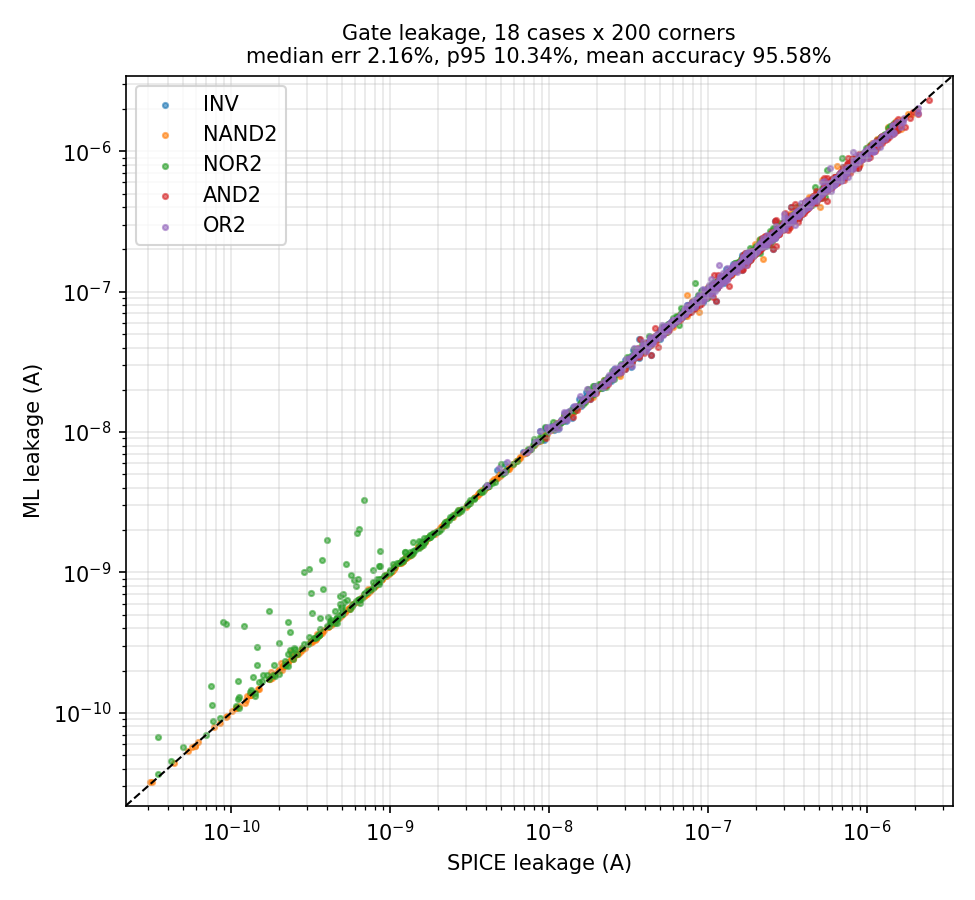
\includegraphics[width=\columnwidth]{gate_parity.png}
\caption{Gate parity plot: ML vs SPICE leakage for all 18 cases $\times$ 200 corners (varying widths), version A (left) and B (right).}
\label{fig:gateparity}
\end{figure}

\textbf{Most accurate} (version A, $\ge99\pct$, 9 cases): NAND2 00 (99.55\pct), NAND2 10 (99.49\pct),
NOR2 10 (99.44\pct), OR2 10, NAND2 01, NOR2 00, INV 0, OR2 11 and OR2 01. Their leakage is carried
by an OFF device in a well-sampled region, e.g.\ a stacked OFF NMOS, or an OFF PMOS with both ends
near $V_{DD}$.

\textbf{Least accurate}: NOR2 11 (96.28\pct) and OR2 00 (97.67\pct), then the cases in which an OFF
PMOS holds the full supply (source at $V_{DD}$, drain at 0: INV 1, NAND2 11, AND2 00, NOR2 01;
98.2--98.4\pct). The reasons are analysed in Section~\ref{sec:err}.

The ML captures the strong input-pattern dependence: NAND2 leaks 650$\times$ less with both
inputs at 0 than with both at 1 (stacking effect), and version A predicts both patterns within
0.13\pct{} bias.

\begin{figure}[!htbp]
\centering
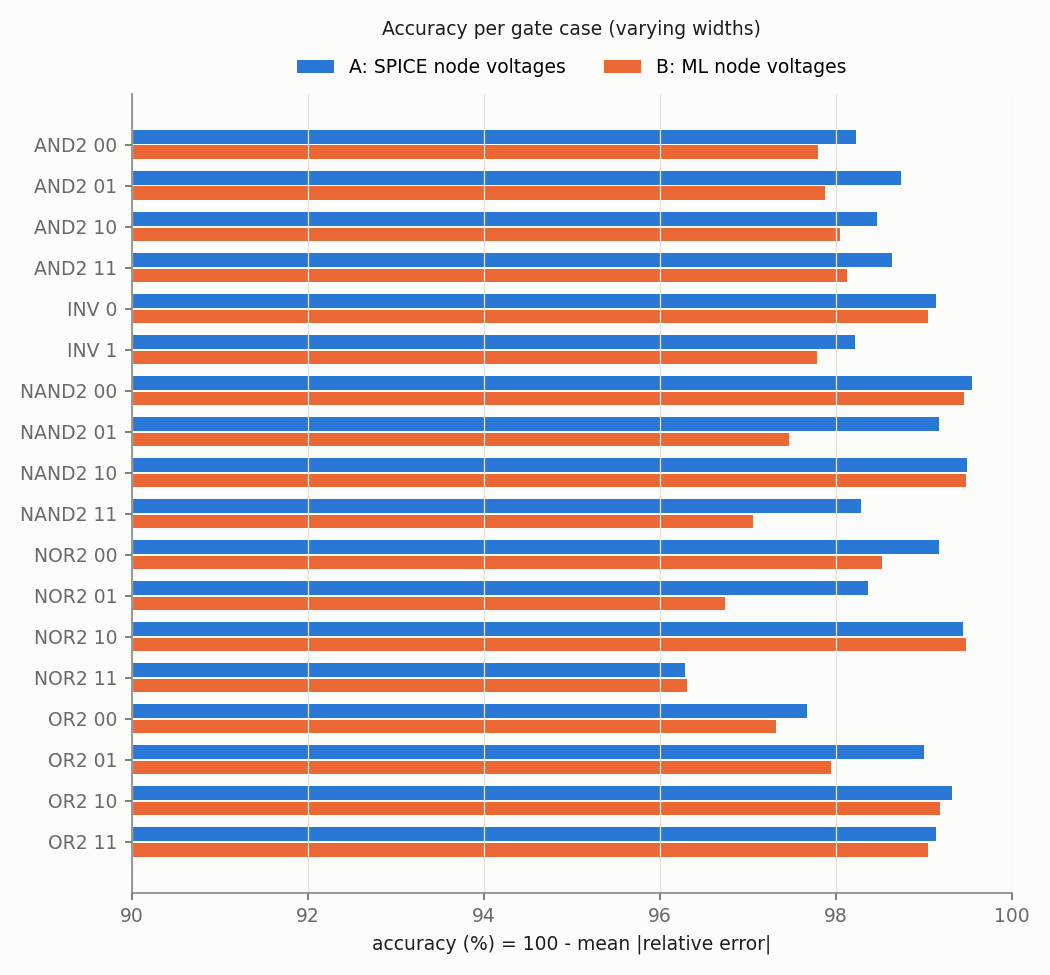
\includegraphics[width=0.92\columnwidth]{gate_accuracy_by_case.png}
\caption{Accuracy of each gate case, versions A and B (varying widths).}
\label{fig:gatecase}
\end{figure}

\textbf{Version B.} ML-solved internal nodes between the rails agree with SPICE within
$\approx$0.5\,mV median (worst 3--5\,mV), e.g.\ NAND2 00 node $x$: 0.1509\,V (SPICE) vs 0.1507\,V
(ML). Nodes driven to a rail come out exactly at the rail, while SPICE places them up to
$\approx$1.4\,mV (median) away: the models do not resolve the ON channel below $\approx$2\,mV, so
the ON device acts as an ideal switch. An OFF device attached to such a node sees a slightly larger
$V_{gs}$ or $V_{ds}$; since sub-threshold current is exponential in both, a 0.6\,mV shift gives
$e^{0.6\,\text{mV}/nV_t}\approx+1.7\pct$. This explains the $+0.8$ to $+1.7\pct$ bias of NAND2
01/11, NOR2 01 and OR2 01 in version B.

% =====================================================================
\section{Test-Circuit Results}

The parity checker is a balanced tree of seven XOR2 gates, each made of four NAND2
($n_1=\overline{ab}$, $n_2=\overline{a n_1}$, $n_3=\overline{b n_1}$, $out=\overline{n_2 n_3}$):
28 NAND2 and 112 transistors. SPICE simulates the complete netlist for all 256 input vectors at
the same 200 corners (51,200 simulations, no failures, every output correct). For the ML
prediction, a logic simulation gives the two inputs of every NAND2, the Part~B NAND2 leakage
(version A or B) is taken for that pattern and corner, and the 28 values are summed.

\begin{table}[!t]
\caption{Parity checker results (256 vectors $\times$ 200 corners = 51,200). Medians in $\mu$A; errors in \%}
\label{tab:circuit}
\centering
\footnotesize
\setlength{\tabcolsep}{3.2pt}
\begin{tabular}{@{}lcccccc@{}}
\toprule
Version & SPICE med & ML med & Bias & Med & p95 & \textbf{Acc}\\
\midrule
A: SPICE node voltages & 7.603 & 7.445 & $-$2.29 & 2.50 & 8.18 & \textbf{96.91}\\
B: ML node voltages & 7.603 & 7.506 & $-$0.96 & 2.14 & 7.88 & \textbf{97.08}\\
\midrule
\multicolumn{7}{@{}l}{Gate-summation limit (SPICE NAND2 sum vs SPICE circuit):}\\
\multicolumn{7}{@{}l}{97.28\pct{} accuracy, bias $-2.21\pct$}\\
\bottomrule
\end{tabular}
\end{table}

\begin{figure}[!htbp]
\centering
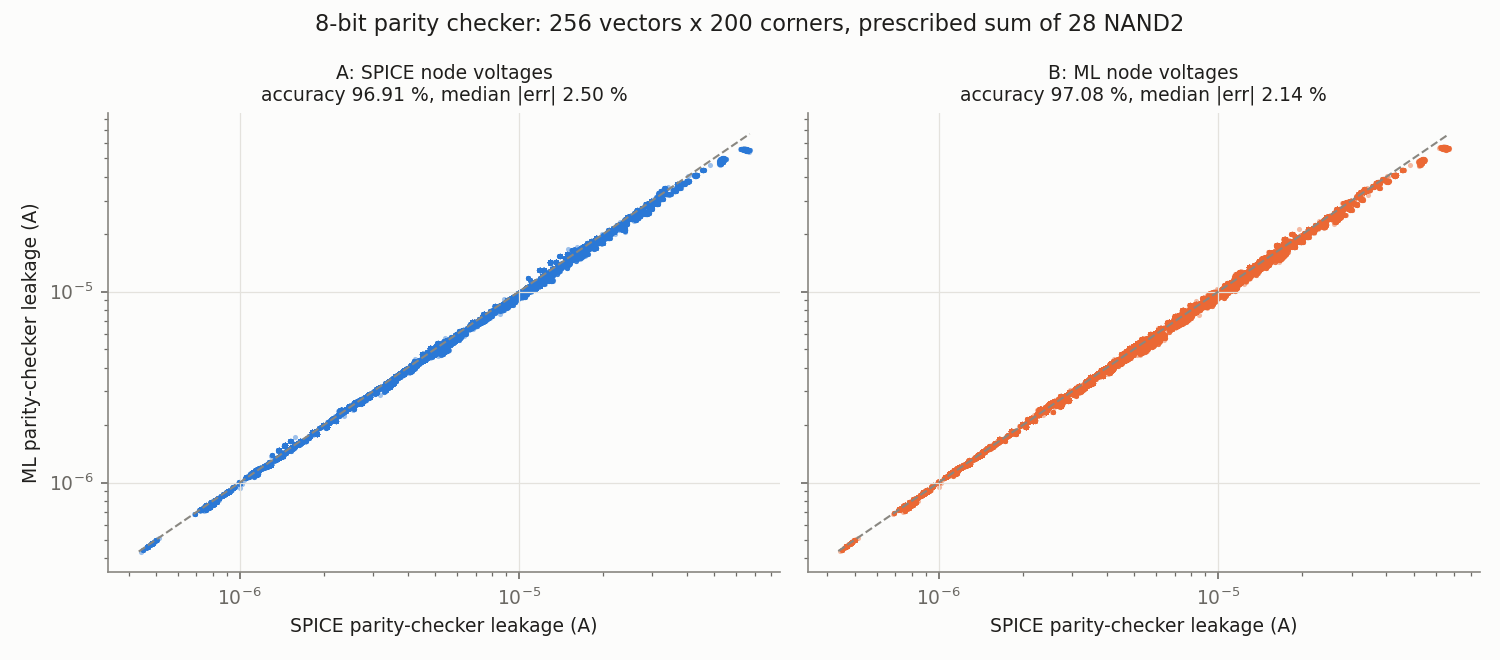
\includegraphics[width=\columnwidth]{circuit_parity.png}
\caption{Parity checker: ML vs SPICE leakage, 256 vectors $\times$ 200 corners, version A (left) and B (right).}
\label{fig:circuitparity}
\end{figure}

\begin{figure*}[!t]
\centering
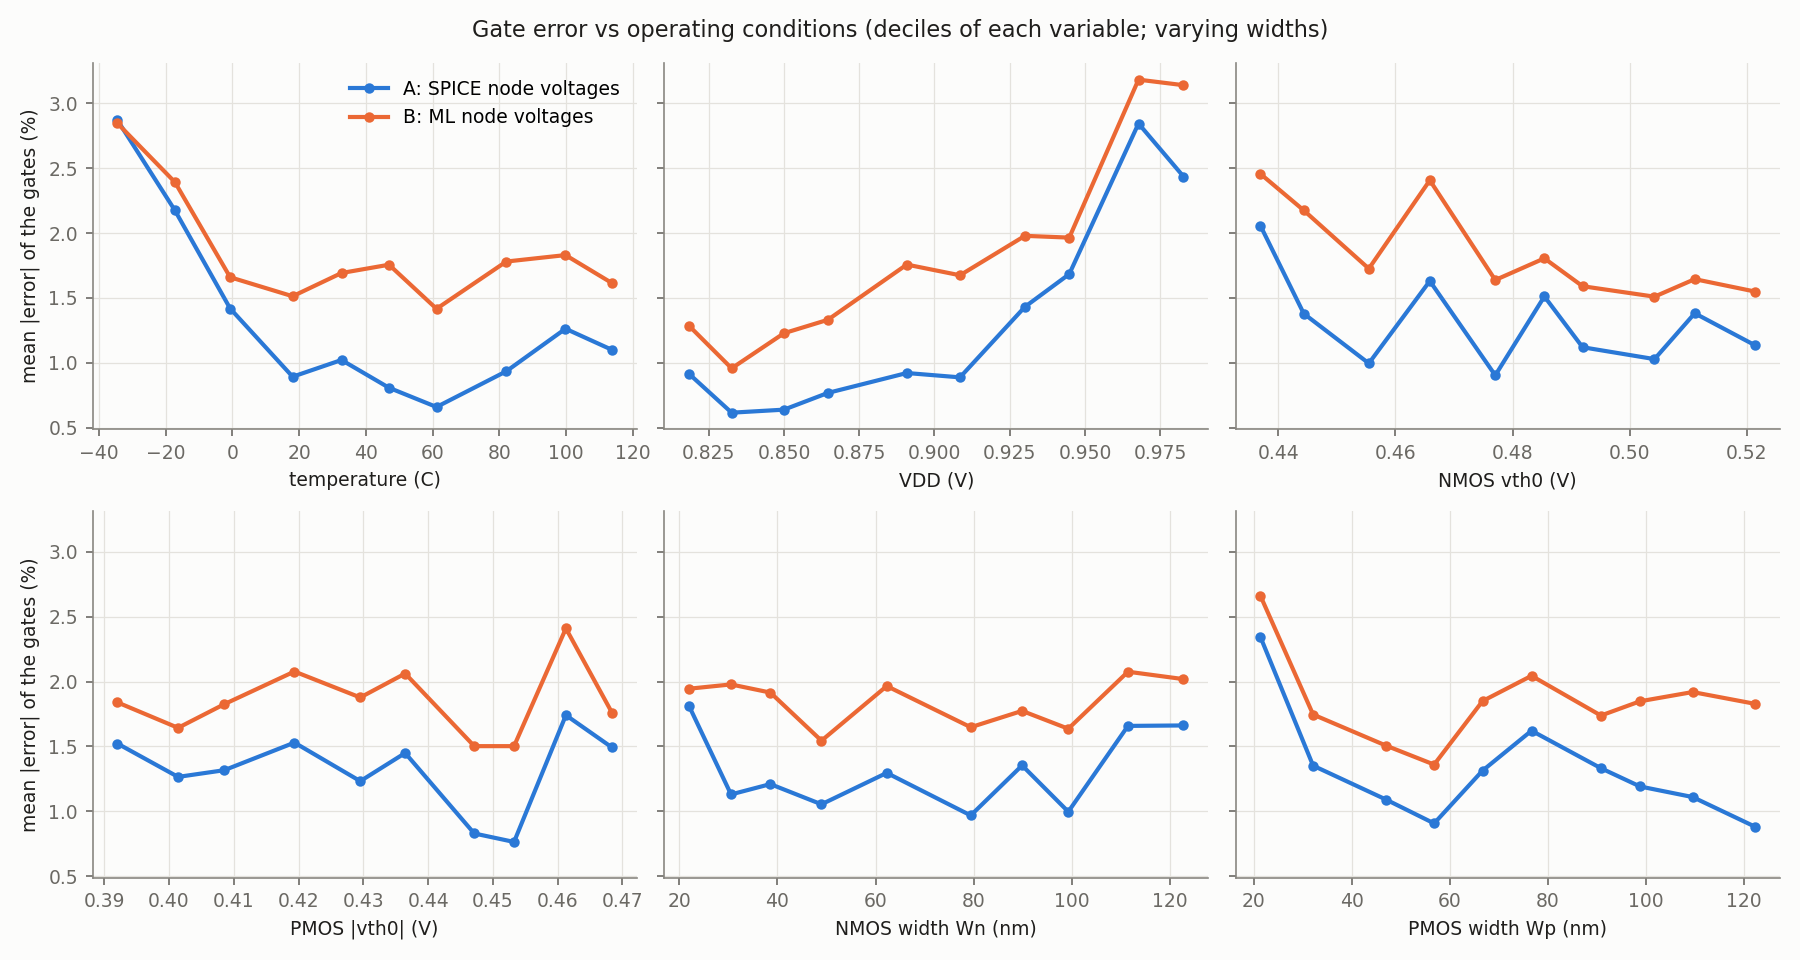
\includegraphics[width=0.9\textwidth]{error_vs_conditions.png}
\caption{Mean $|$error$|$ of all gate cases per decile of each corner variable (version A blue, B orange; varying widths).}
\label{fig:cond}
\end{figure*}

Table~\ref{tab:circuit} and Fig.~\ref{fig:circuitparity} give the results. The circuit leakage
(0.44--67\,$\mu$A) is predicted with \textbf{96.91\pct} accuracy in version A and
\textbf{97.08\pct} in version B. Accuracy is 96.0--97.1\pct{} for every number of ones in the input
vector, so no input class is badly predicted.

\textbf{Comparison with the gates.} The circuit is 1.8 points below the gates (96.91 vs
98.69\pct, version A), as the project document anticipates. To separate the ML error from the
method, we summed the \emph{SPICE} leakages of the 28 stand-alone NAND2 and compared them with the
SPICE circuit: even with perfect gate models the summation reaches only 97.28\pct, with a bias of
$-2.21\pct$. The ML bias of version A ($-2.29\pct$) is almost exactly this composition bias, so
nearly all of the circuit error comes from the prescribed summation, not from the models. Version
B scores higher only because its $+1\pct$ NAND2 bias (Section~IV) partly cancels the composition
bias; it is not a better circuit method.

% =====================================================================
\section{Error Analysis}
\label{sec:err}

\textbf{By transistor case.} PMOS OFF has the largest transistor-level errors, all at the
$\sim10^{-14}$\,A noise floor: its channel current falls about 10$\times$ per 50\,mV as the source
moves away from $V_{DD}$, so most random samples end up at the floor. 16nm\_HP makes this extreme:
among the eleven course model cards it has the highest leakage (6.85\,$\mu$A/$\mu$m at 25$^\circ$C,
2.6$\times$ the next) and only 0.07\pct{} gate current, so a pinched-off channel leaves almost
nothing above the noise. (On the same cards, the LP and MGK files have 53--99\pct{} gate current;
for 16nm\_HP sub-threshold leakage dominates.)

\textbf{By gate and input.}
\begin{itemize}
\item \emph{NOR2 11} (96.28\pct): both inputs at 1, so the PMOS stack is off and, at cold corners,
barely leaks; the leakage is then almost only the gate current of the two ON NMOS with 0\,V across
them. That operating point is rare in uniform training data (0.3\pct{} of rows have $V_d,V_s<50$\,mV).
Mean $|e|$ is 6.1\pct{} below 0$^\circ$C and 2.9\pct{} above, and 9 of the 10 largest gate errors
(+16 to +26\pct) are NOR2 11. The plain-voltage features already removed most of this error: in a
direct single-transistor SPICE check at this operating point, the ON-NMOS gate-current error at
cold corners fell from $\approx$100\pct{} to 7\pct{} (median).
\item \emph{OR2 00} (97.67\pct): the NOR output \cc{nr} is a ``1'' through two series ON PMOS and
sags furthest below $V_{DD}$ of all internal nodes (median $\approx$10\,mV). The INV stage's OFF
PMOS sees this sag as gate drive. Using the real gate voltage reduced this error from 93.7\pct{} to
97.7\pct; the remaining $+1.3\pct$ bias, and the single worst gate prediction ($+33\pct$ at
97$^\circ$C, $V_{DD}=0.99$\,V), occur where the off-rail gate takes the PMOS OFF model outside its
training data (gate exactly on the rail).
\item \emph{OFF PMOS holding the full supply} (INV 1, NAND2 11, AND2 00, NOR2 01): source at
$V_{DD}$ and drain at 0 is a sparsely sampled corner of the PMOS OFF input space.
\end{itemize}

\textbf{By corner condition} (Fig.~\ref{fig:cond}, version A):
\begin{itemize}
\item \emph{Cold} ($\approx-35^\circ$C): 2.9\pct{} mean $|e|$ against 0.7--1.3\pct{} above 0$^\circ$C.
Leakage is smallest, so the gate-current-dominated NOR2 11 and the full-supply PMOS OFF cases
(3.7--3.9\pct{} below 0$^\circ$C vs $\approx$1\pct{} above) dominate.
\item \emph{High $V_{DD}$} (0.97--0.99\,V): 2.8\pct{} vs 0.6--1.7\pct{}. The edge of a uniform
range has the fewest training neighbours, and internal nodes sag most there.
\item \emph{Narrow PMOS} ($W_p\approx21$\,nm): 2.3\pct{} vs 0.9--1.6\pct{}; with $W_n/W_p>3$ the
full-supply PMOS OFF cases reach 4.1--4.3\pct{} (1.5--1.6\pct{} otherwise). A weak OFF PMOS against
a strong ON NMOS sits at the bottom edge of the width range.
\item \emph{Low NMOS vth0} ($\approx$0.437\,V, $-9\pct$): 2.1\pct{} vs 0.9--1.6\pct; the leakiest
NMOS corners at the edge of the \cc{vth0} range.
\end{itemize}
PMOS $|$\cc{vth0}$|$ and $W_n$ show no monotonic trend. Version B follows the same pattern about
0.5 points higher. For the \emph{circuit}, the error instead grows with temperature: the version-A
bias is $-0.8\pct$ in the coldest fifth of the corners and $-4.6\pct$ in the hottest, because the
composition effect (Section~V) scales with leakage: a logic~1 produced by a NAND2 sits below
$V_{DD}$ by the leakage drop across its ON PMOS, and the OFF PMOS it drives leaks exponentially
more.

% =====================================================================
\section{Limitations and Improvements}

\textbf{Limitations.}
\begin{enumerate}
\item \emph{Gate summation.} Ideal 0/$V_{DD}$ inputs and no loading cap the circuit at
$\approx$97.3\pct{} on this card (bias $-2.2\pct$, worse when hot); our 96.91\pct{} is close to it.
\item \emph{Rail nodes in version B.} The models do not resolve an ON channel below
$\approx$2\,mV, which biases some stacked cases by 1--2\pct.
\item \emph{Rare operating points}: ON-NMOS gate current at $V_{ds}=0$ (NOR2 11), the full-supply
PMOS OFF point, and the edges of the $V_{DD}$, $W$ and \cc{vth0} ranges carry 2--4\pct{} error.
\item \emph{Gate voltage on the rail.} The training data fixes the gate at 0 or $V_{DD}$ (the
document's case definition). Off-rail gates (AND2/OR2 INV stage) are extrapolated; retraining with
40,000 extra off-rail rows per case made the validation error worse in all four cases
(e.g.\ NMOS ON 0.31$\to$0.97\pct), so it was not adopted.
\item \emph{Cost.} Each averaged GP trains in $\approx$15\,min; the version-B node solver needs
$\approx$1--2\,h for 3,600 gate evaluations on four cores.
\end{enumerate}

\begin{table}[!t]
\caption{Optional extension (not the prescribed method): voltage-aware parity checker, varying widths}
\label{tab:vparity}
\centering
\footnotesize
\begin{tabular}{@{}lcccc@{}}
\toprule
Method & Acc & Med & p95 & Bias\\
\midrule
Prescribed summation, A & 96.91 & 2.50 & 8.18 & $-$2.29\\
Prescribed summation, B & 97.08 & 2.14 & 7.88 & $-$0.96\\
Depth 0: ideal inputs, linear ON current & 96.41 & 3.04 & 8.56 & $-$2.83\\
\textbf{Depth 1: driver output voltages} & \textbf{98.24} & \textbf{1.18} & \textbf{5.39} & \textbf{+0.40}\\
\bottomrule
\end{tabular}
\end{table}

\textbf{Improvements.}
\begin{enumerate}
\item \emph{Voltage-aware composition} (implemented as an optional extension, Table~\ref{tab:vparity}):
each NAND2 input driven by another NAND2 gets that driver's ML-predicted output voltage instead of
an ideal level, and ON devices below 2\,mV get a linear-region channel current. The parity checker
then reaches \textbf{98.24\pct} (bias $+0.40\pct$), above the 97.28\pct{} limit of the prescribed
summation. Modelling the input current drawn by the receiving gate (loading) is the next step.
\item A linear-region ON model below 2\,mV for version B of the gates, to remove the rail-node
bias.
\item Targeted instead of uniform extra data: ON NMOS near $V_d=V_s=0$, PMOS OFF near
source\,=\,$V_{DD}$, drain\,=\,0, and the edges of the $V_{DD}$, $W$ and \cc{vth0} ranges.
\item Off-rail gate data as a separate expert rather than mixed into the main training pool.
\item Faster models (sparse GPs, or distilling the GP into a small network) for larger circuits.
\end{enumerate}

\FloatBarrier
% =====================================================================
\section{Conclusion}
Transistor models trained only on single-device SPICE data predict gate leakage under PVT and
width variation with 98.69\pct{} mean accuracy (98.15\pct{} without any SPICE node voltages), and
the 8-bit parity checker with 96.91\pct{} (97.08\pct). The circuit error is set by the prescribed
gate-summation method ($-2.2\pct$ composition bias on 16nm\_HP); passing real gate output voltages
between gates lifts the circuit to 98.24\pct.

\newpage
\section*{Team Contributions}
The work was shared equally (25\pct{} each):

\begin{center}
\footnotesize
\setlength{\tabcolsep}{3pt}
\begin{tabular}{@{}p{0.27\columnwidth}p{0.70\columnwidth}@{}}
\toprule
Member & Work\\
\midrule
Bhargav\newline(2023112014) & Part A models: preprocessing and physics features, comparison of the four model types, averaged GP, final models and dataset-size study\\
Nitin\newline(2023112026) & Simulation setup and Part A data: ngspice flow, sampling, netlists, the 10,000-row and extra datasets, Kirchhoff check and trend plots\\
Karthik\newline(2023102009) & Part B gates: corners and widths, gate SPICE, cut-set leakage, versions A and B (ML node solver), real gate voltage\\
Roshan Lal\newline(2023102010) & Part C and analysis: parity-checker SPICE and composition, error analysis, voltage-aware extension, reproducibility and report\\
\bottomrule
\end{tabular}
\end{center}

\appendices
\section{Deliverables and Reproducibility}
All code, data and results are available at
\url{https://github.com/saiXbhargav/DVD_Project}.
\cc{run\_all.sh} runs ten scripts in order with fixed seeds (data 2026--2029, extra data
5001--5304 and 7001--7304, split 42, models 7, corners 1234, widths 2468);
\cc{verify\_final.py} checks inputs against SHA-256 hashes and every result table against the
reference outputs (all identical). The model files (145\,MB) and extra training rows (84\,MB) are
kept outside the repository, hashed in \cc{MANIFEST.sha256}, and regenerated by steps 1 and 3.

\begin{table}[!h]
\caption{Deliverables (project document, Section 6)}
\label{tab:deliv}
\centering
\footnotesize
\setlength{\tabcolsep}{3pt}
\begin{tabular}{@{}p{0.27\columnwidth}p{0.70\columnwidth}@{}}
\toprule
Deliverable & Location (repository)\\
\midrule
1 Datasets & \cc{data/\{nmos,pmos\}\_\{on,off\}.csv}\\
2 Example netlists & \cc{netlists/*\_example.cir}, \cc{gate\_*\_w.cir}, \cc{parity8\_w.cir}\\
3 Data check & \cc{results/kcl\_check.csv}, \cc{figures/trend\_*.png}\\
4 Model comparison & \cc{results/model\_comparison\_val.csv}\\
5 Chosen models & \cc{results/transistor\_metrics.csv}, \cc{figures/pred\_vs\_spice\_*.png}, \cc{models\_trained/*.joblib}\\
6 Gate results & \cc{results/gate\_results.csv}; per case and corner: \cc{results/gate\_ml.csv}\\
7 Gate parity plot & \cc{figures/gate\_parity.png}\\
8 Test circuit & \cc{results/circuit\_results.csv}, \cc{figures/circuit\_parity.png}\\
9 Code & \cc{01\_}\ldots\cc{10\_*.py}, \cc{final\_method.py}, \cc{run\_all.sh}\\
\bottomrule
\end{tabular}
\end{table}

\FloatBarrier
\begin{thebibliography}{9}
\bibitem{roy03} K.~Roy, S.~Mukhopadhyay and H.~Mahmoodi-Meimand, ``Leakage current mechanisms and
leakage reduction techniques in deep-submicrometer CMOS circuits,'' \emph{Proc. IEEE}, vol.~91,
no.~2, pp.~305--327, 2003.
\bibitem{ptm} Predictive Technology Model (PTM), Arizona State University,
\url{https://ptm.asu.edu}.
\bibitem{bsim4} BSIM4 MOSFET model user's manual, BSIM Group, UC Berkeley.
\bibitem{ngspice} ngspice: open-source mixed-signal circuit simulator,
\url{https://ngspice.sourceforge.io}.
\bibitem{gp} C.~E.~Rasmussen and C.~K.~I.~Williams, \emph{Gaussian Processes for Machine
Learning}. MIT Press, 2006.
\bibitem{sklearn} F.~Pedregosa \emph{et al.}, ``Scikit-learn: machine learning in Python,''
\emph{J. Mach. Learn. Res.}, vol.~12, pp.~2825--2830, 2011.
\bibitem{lgbm} G.~Ke \emph{et al.}, ``LightGBM: a highly efficient gradient boosting decision
tree,'' in \emph{Proc. NeurIPS}, 2017.
\end{thebibliography}

\end{document}
